\documentclass[lang=cn]{elegantpaper}
\usepackage{ulem}
\usepackage{wrapfig}

\title{\textbf{Atomic Student Manager Reborn 系统使用指南}}
\author{作者:XYCode}
\version{\uline{0.0.1-alpha.1} document}

\def\equationautorefname{式}%
\def\footnoteautorefname{脚注}%
\def\itemautorefname{项}%
\def\figureautorefname{图}%
\def\tableautorefname{表}%
\def\partautorefname{篇}%
\def\appendixautorefname{附录}%
\def\chapterautorefname{章}%
\def\sectionautorefname{节}%
\def\subsectionautorefname{小小节}%
\def\subsubsectionautorefname{subsubsection}%
\def\paragraphautorefname{段落}%
\def\subparagraphautorefname{子段落}%
\def\FancyVerbLineautorefname{行}%
\def\theoremautorefname{定理}%

\begin{document}
\maketitle

\tableofcontents

\section{什么是 Atomic Student Manager Reborn}
    \uline{A}tomic \uline{S}tudent \uline{M}anager \uline{Re}born,简称为 ASMRE,是 Atomic Student Manager 项目的完全重构。是一个采用了Nuxt、SSR、FaaS、Kubernetes等前沿技术制作的学生管理系统。

    相较于ASMRE的前辈ASM,ASMRE最大的特点是实现了多班级支持和多端可用,允许为每个学生创建账号以便他们监督或对班委的工作提出意见。
    并且,ASMRE\textbf{不但可以管理学生的操行分(见 \autoref{section:操行分管理})\footnote{您可以理解为学分,反正我们学校是叫操行分。},还支持家庭作业管理(见 \autoref{section:家庭作业管理})、为学生分配任务等(见 \autoref{section:学生任务管理})。}。
    而且,ASMRE有着严格的权限管理,我们使用Casbin自带的Casbin-RBAC权限模型来实现精细化的权限控制\footnote{原本计划使用ABAC权限模型,但是由于ABAC的管理需要专人维护,因此没有采用。}

    同时,ASMRE提供了开放且经过严格权限控制的HTTP API供使用,任何人无需申请即可使用该API。我们使用的框架 FastAPI 将会自动生成可视化的 API 文档,方便其他开发者在 ASMRE 的基础上进行拓展。

\section{Atomic Student Manager Reborn 的基本架构}
    ASMRE会预先鉴权,以减少不必要请求的发送,如\autoref{figure:image:鉴权流程}。如果用户在预鉴权阶段就已确认没有该权限,则ASMRE不会显示执行该操作的入口。

    \begin{figure}[htbp]
        \centering
        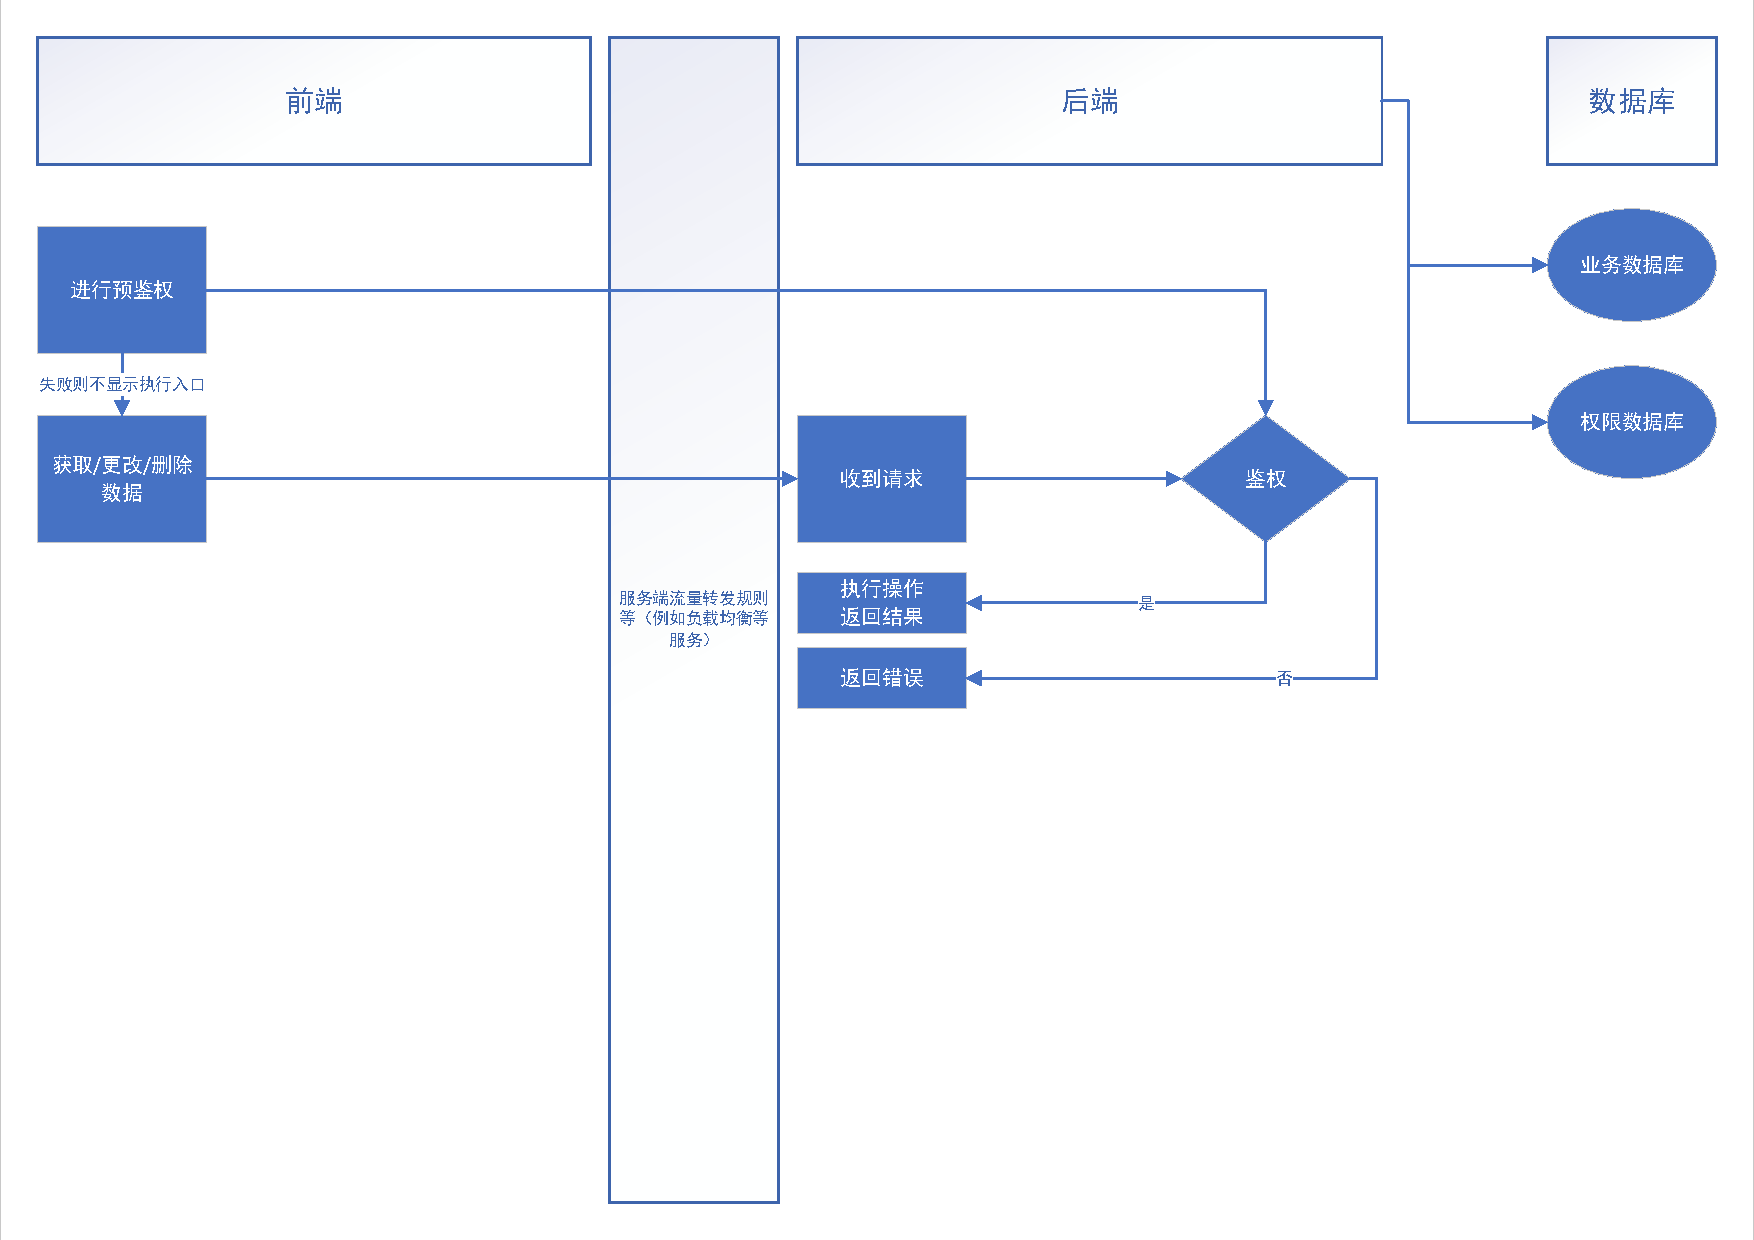
\includegraphics[width=0.75\textwidth]{./figure/images/asmre-request-about-permission.pdf}
        \caption{ASMRE请求流程(关于鉴权)}\label{figure:image:鉴权流程}
    \end{figure}

    ASMRE的一个用户可以绑定多个学生,任务、操行分等属性是对于学生而言的,执行操作(例如更改、获取数据)的主体则是用户。如\autoref{figure:image:关系}。(提示:这是矢量图,在计算机上可以随意放大查看,清晰度不损失)

    \begin{figure}[htbp]
        \centering
        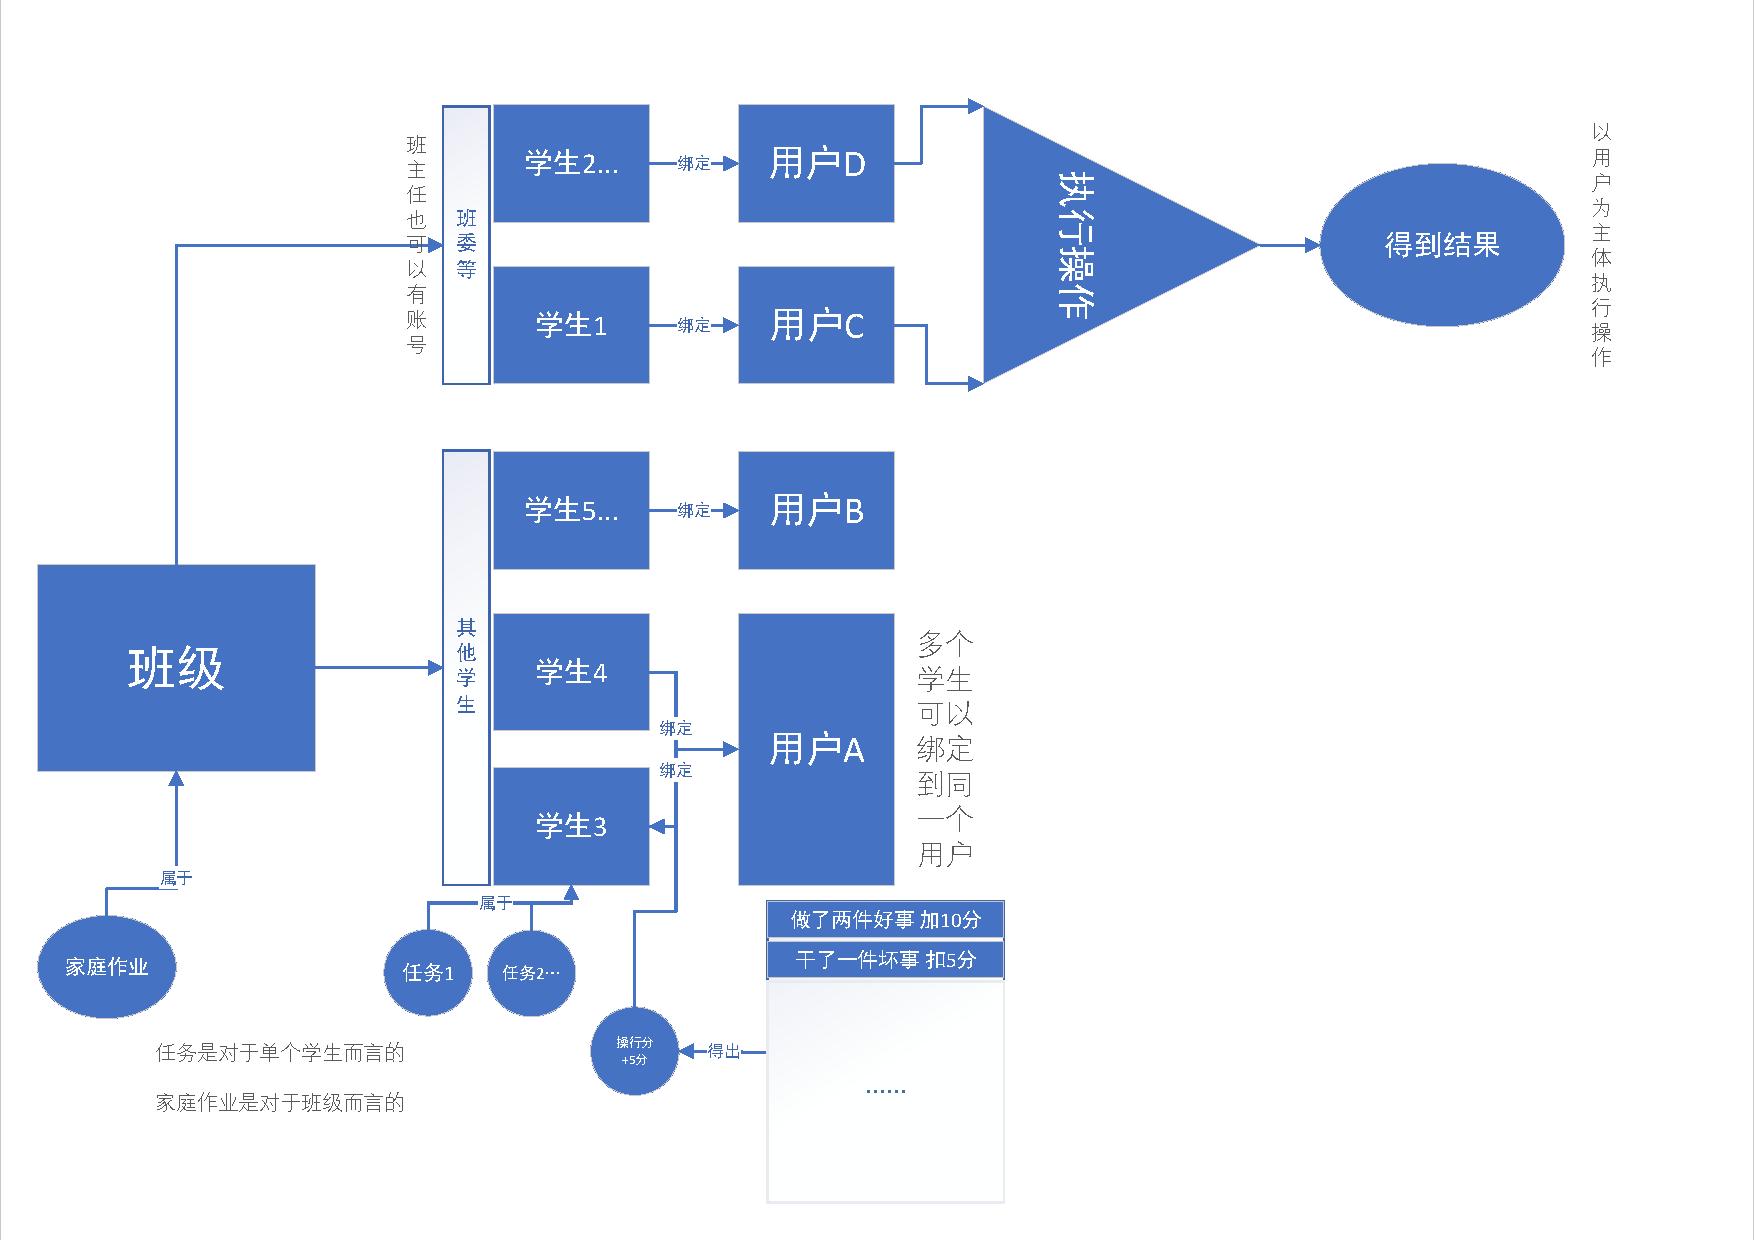
\includegraphics[width=0.5\textwidth]{./figure/images/asmre-bindings.pdf}
        \caption{ASMRE中的各种关系}\label{figure:image:关系}
    \end{figure}

\section{操行分管理}
    \label{section:操行分管理}

    操行分管理是 ASMRE 最基本的功能之一,是其前辈 ASM 实现的唯一功能。在 ASMRE 中,我们为其新增了许多新功能,使得其更加易用。

    \subsection{创建班级和导入学生}
        首先,您需要创建一个班级,这需要您拥有\uline{/asmre/class}资源的\uline{create}权限,如果没有,请联系系统管理员为您的账号开通。\footnote{不要直接修改数据库,请通过 HTTP API 进行修改,否则需要手动重载权限策略(重启后端服务)。}。

        \begin{wrapfigure}[8]{r}{0.6\textwidth}
            \centering
            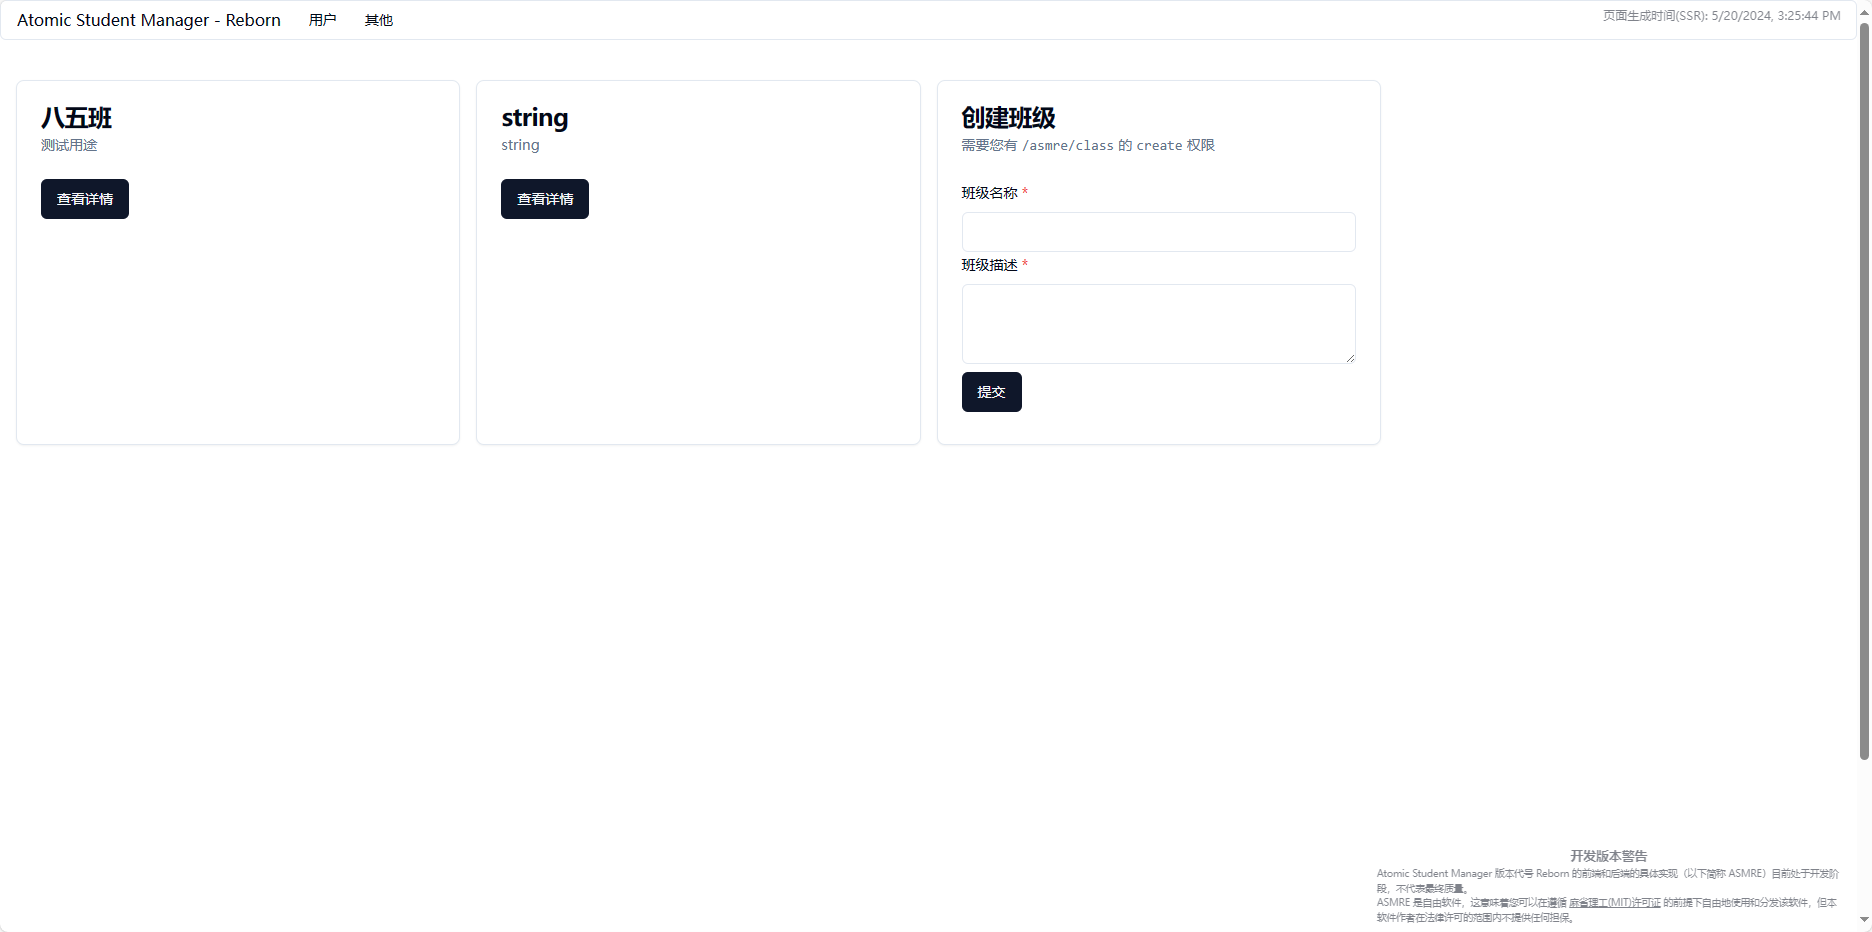
\includegraphics[width=0.5\textwidth]{figure/images/create-class.png}
            \caption{创建班级页面}
            \label{figure:image:创建班级页面}
        \end{wrapfigure}

        如果您正常拥有该权限,应该可以看到\autoref{figure:image:创建班级页面}中第三个格子的内容。

        然后,您可以邀请学生们来手动注册一个账号,然后手动操作数据库将他们绑定到对应的学生上,或者使用一个叫做 MergeASM 的脚本来批量导入,MergeASM脚本的源代码目前托管于\textbf{https://github.com~/XYCode-Kerman/MergeASM}。

        \vspace{0.25cm}

        \textbf{
            邮箱中填入 Gravatar 或 Cravatar 中注册过的邮箱,将会自动返回这两个网站上配置的头像。如果填入QQ邮箱,则返回该QQ号对应的头像。
        }

    \subsection{操作操行分}
        \begin{wrapfigure}[8]{r}{0.4\textwidth}
            \centering
            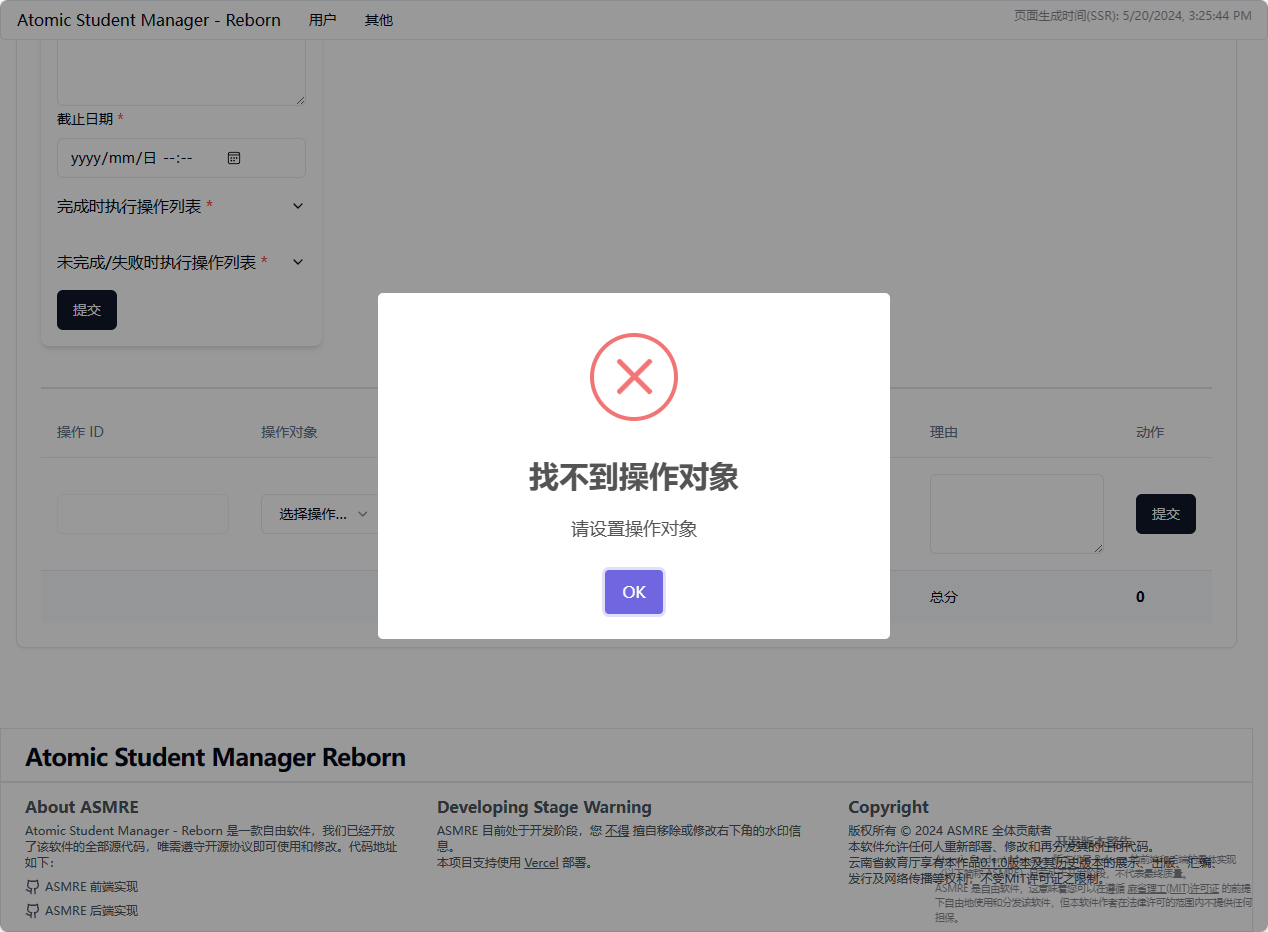
\includegraphics[width=0.35\textwidth]{figure/images/object-not-found.png}
            \caption{找不到操作对象}\label{figure:image:找不到操作对象}
        \end{wrapfigure}

        如果您正常拥有资源\uline{/asmre/credit/student\_name}的create权限,您就可以创建操行分更新记录,如果拥有write和delete权限,您就可以修改和删除操行分更新记录。

        注意!请选择好操作对象再提交,否则会出现\autoref{figure:image:找不到操作对象}中的错误。

\section{家庭作业管理}
    \label{section:家庭作业管理}

    确保您有\uline{/asmre/homework}的create权限,然后您可以点击 \autoref{figure:image:新增家庭作业按钮} 中所示的按钮来\textbf{展开创建作业的表单}。

    \begin{figure}[htbp]
        \centering
        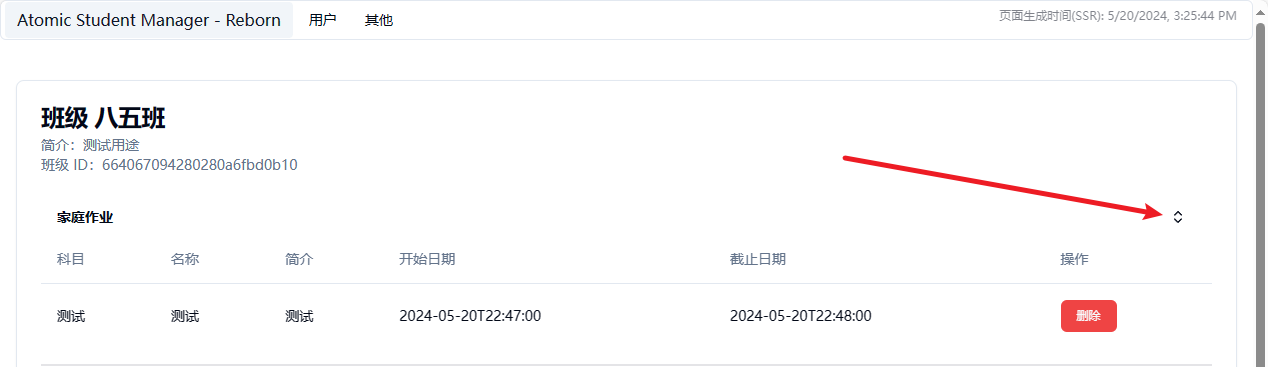
\includegraphics[width=0.75\textwidth]{figure/images/add-homework-btn.png}
        \caption{新增家庭作业按钮}\label{figure:image:新增家庭作业按钮}
    \end{figure}

    点击 \autoref{figure:image:新增家庭作业按钮} 中的删除按钮可以删除一项作业。

\section{学生任务管理}
    \label{section:学生任务管理}

    学生任务和家庭作业大体上是相同的,但\textbf{学生任务是针对于单个学生而非全班的}。通常用作给学生布置其他工作或者执行其他处罚(例如罚扫地、抄班规等)。

    例如\autoref{figure:image:任务示例}中的这位同学,因为\textit{第三节晚自习在自习室打闹,被其他班老师点名批评},被处罚\textit{抄班规}。班委要求他在\textit{2024/5/22 23:59:00}之前完成。目前的状态是\textit{进行中}(截图于 2024年5月21日 00点40分)。

    班委设置了一个\textit{未完成/失败时动作},内容为\textit{扣除5分操行分},这代表如果他没有在规定时间内完成该任务,班委\textbf{有正当理由(注意不是自动扣除)}扣除其的5分操行分。

    如果是非惩罚性质的,还可以设置\textit{完成时动作},内容可以为加分等。

    \textbf{您可以同时设置多个“动作”。}

    \begin{figure}[htbp]
        \centering
        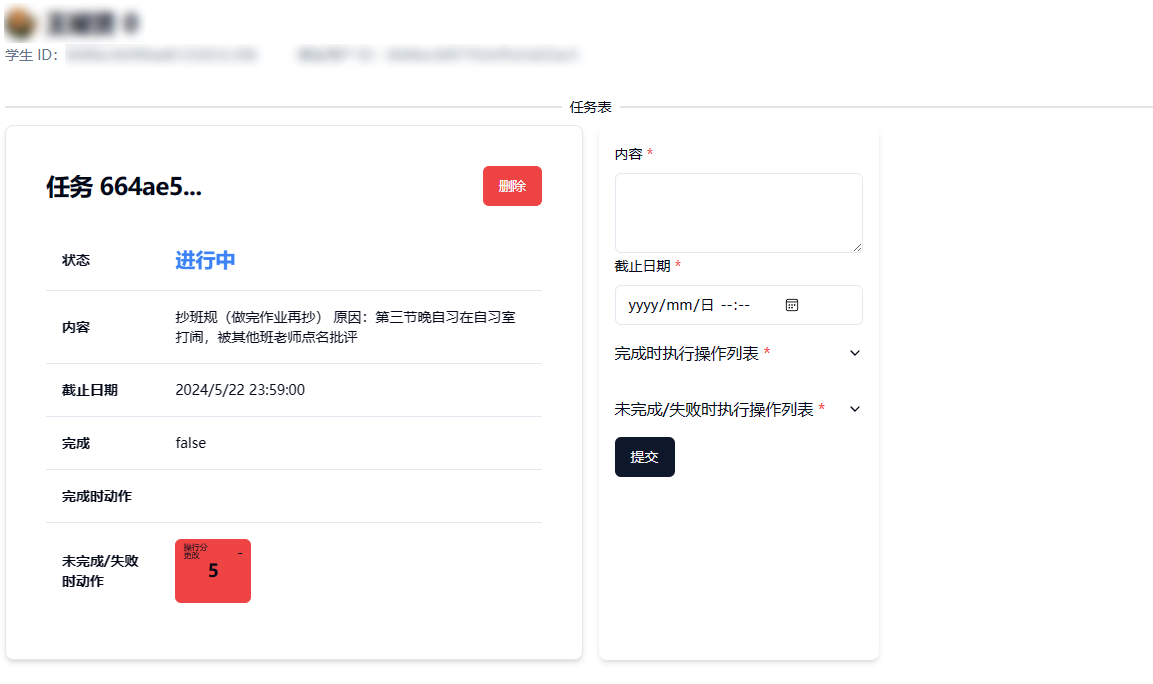
\includegraphics[width=0.9\textwidth]{figure/images/task-example.png}
        \caption{任务示例}\label{figure:image:任务示例}
    \end{figure}

\end{document}